\documentclass[letter,12pt]{article}
\usepackage[utf8]{inputenc}
%\usepackage[spanish]{babel}
\decimalpoint
\pagenumbering{gobble}
\usepackage{listings}

%opening
\title{Una aproximación a $sen(x)$}
\author{Luis Enrique Serrano Gutiérrez}
\usepackage{tikz,stackengine}
\usepackage{pgfplots}


\newcommand{\EnmarcaSL}[1]{\begin{center}\fbox{#1}\end{center}}
\newcommand{\Enmarca}[1]{{\centering\fbox{#1}\par}}


\begin{document}

\maketitle


\begin{abstract}
Se presenta una forma de calcular el seno de un número basada en la publicación ''Algoritmos Sencillos para Evaluar Funciones Elementales''escrita por el profesor Pablo Barrera Sánchez \cite{AlgoritmosPablo}.
\end{abstract}

\section*{Las ideas}
La base para este procedimiento son los siguientes dos hechos: 
\begin{enumerate}
	\item $\lim_{x\to 0} \frac{sen(x)}{x} = 1$\\\\	
Esto quiere decir que para valores de $\alpha$ muy cercanos a cero el seno($\alpha$) es muy cercano a $\alpha$, por ejemplo:
	\begin{table}[h!]
		\centering
		\begin{tabular}{ |c|c|c|c| } 
		  \hline
		 	i & $\alpha = 1/i^i$ & sen($\alpha)$ & $\alpha - $sen($\alpha)$ \\
		  \hline
			1 & 0.500000000000 & 0.479425538604 & -0.020574461396\\
			2 & 0.250000000000 & 0.247403959255 & -0.002596040745\\
			3 & 0.125000000000 & 0.124674733385 & -0.000325266615\\
			4 & 0.062500000000 & 0.062459317842 & -0.000040682158\\
			5 & 0.031250000000 & 0.031244913985 & -0.000005086015\\	  
		 \hline
		\end{tabular}
	\caption{Comparación $sen(\alpha)$ contra $\alpha$ para valores de $\alpha$ cercanos a cero}
	\label{table:1}
	\end{table}	
	\enlargethispage*\baselineskip{}
	\item $sen(2\alpha)=2sen(\alpha)\sqrt{1-sen^2(\alpha)}$\\\\
	Este hecho se deduce de las identidades:\\\\
	$sen(2\alpha)=2sen(\alpha)cos(\alpha)\\
	sen^2(\alpha)+cos^2(\alpha)=1$
\end{enumerate}

\pagebreak
\section*{El procedimiento}
\ifx
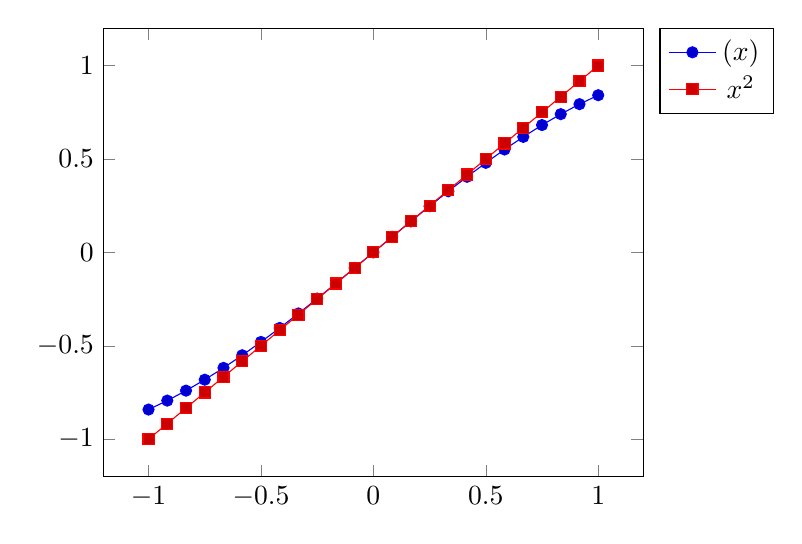
\begin{tikzpicture}
    \begin{axis}[domain=-1:1,legend pos=outer north east]
    \addplot {sin(deg(x))}; 
    \addplot {x};
    \legend{$\sen(x)$,$x^2$}
    \end{axis}
\end{tikzpicture}\\\\
\fi
\ifx
El valor más grande de $\alpha$ al que se calculará el seno será $2\pi$, dado que el seno es una función periódica de periodo $2\pi$.\fi 
\ifx
https://oeis.org/wiki/List_of_LaTeX_mathematical_symbols
\fi
Si se encuentra la forma de llevar el valor $\alpha$ lo suficientemente cerca a cero se tendría la posibilidad de aplicar la idea del punto 1, ese nuevo valor cercano a cero(que se calcula a partir de $\alpha$) se llamará $\beta$ y se define como: 
$\beta=\frac{\alpha}{2^{5}}$.\\
Este valor es lo suficientemente pequeño para que: $sen(\beta)\approx\beta$. 
\\\\
Por ejemplo, si $\alpha=0.1$ el valor de $\beta$ se calcula de la siguiente forma: $\beta=\frac{\alpha}{2^{5}}=\frac{0.1}{2^{5}}=\frac{0.1}{32}=0.003125$. Para el valor $\beta=0.003125$ se cumple que $sen(\beta)\approx\beta$ para verificarlo se debe calcular la diferencia entre $sen(0.003125)$ y $0.003125$.


{
\centering
\framebox{$sen(\beta)\approx0.003125$}\par
}

Ahora se conoce el valor de $sen(\beta)$ pero el problema original es calcular $sen(\alpha)$ por lo que para ''regresar'' al valor original se hace uso del punto dos, te tal forma que:

$sen(2\beta)=2*sen(\beta)*\sqrt{1-sen^2(\beta)}=\\
2*(0.003125)*\sqrt{1-(0.003125)^2}=\\
0.00625*\sqrt{1-0.000009}=\\
0.00625*\sqrt{0.9999902}=\\
0.00625*0.9999951=0.006250$

\Enmarca{$sen(2\beta)=0.006250$}

Se ha obtenido en forma numérica el valor de $sen(2\beta)$, observemos lo siguiente:
$sen(2\beta)=sen(2\frac{\alpha}{2^{5}})=sen(\frac{\alpha}{2^{5-1}})=sen(\frac{\alpha}{2^{4}})$ el exponente del denominador se redujo en 1, de 5 a 4, por lo que se está una potencia más cerca del valor original. \\
Ahora se calcula el seno del doble del ángulo anterior, $2\beta$

$sen(2(2\beta))=2*sen(2\beta)*\sqrt{1-sen^2(2\beta)}=
\\2*(0.006250)*\sqrt{1-(0.006250)^2}=\\
0.0124999*\sqrt{1-0.0000391}=\\
0.0124999*\sqrt{0.9999609}=\\
0.0124999*0.9999805=0.0124997$\\
$sen(2(2\beta))=0.0124997$

\Enmarca{$sen(2\cdot2\beta)=0.0124997$}
\enlargethispage\baselineskip
\enlargethispage\baselineskip


%\newpage
Observe lo siguiente:
$sen(2(2\beta))=sen(2\frac{\alpha}{2^{4}})=sen(\frac{\alpha}{2^{4-1}})=sen(\frac{\alpha}{2^{3}})$, y nuevamente se esta una potencia más cerca del valor original, por lo que al calcular el seno del doble del ángulo anterior tres veces más se tendrá el seno de $\alpha$ que es el objetivo.

Ahora se calcula el seno del doble del ángulo anterior, $2\cdot2\beta$\\

$sen(2(2\cdot2\beta))=2*sen(2\cdot2\beta)*\sqrt{1-sen^2(2\cdot2\beta)}=
\\2*(0.0124997)*\sqrt{1-(0.0124997)^2}=\\
0.0249994*\sqrt{1-0.0001562}=\\
0.0249994*\sqrt{0.9998438}=\\
0.0249994*0.9999219=0.0249974$\\
$sen(2(2\cdot2\beta))=0.0249974$
 
\Enmarca{$sen(2\cdot2\cdot2\beta))=0.0249974$} 

y, nuevamente: $sen(2(2\cdot2\beta))=sen(2\frac{\alpha}{2^{3}})=sen(\frac{\alpha}{2^{3-1}})=sen(\frac{\alpha}{2^{2}})$

Ahora se calcula el seno del doble del ángulo anterior, $2\cdot2\cdot2\beta$\\

$sen(2(2\cdot2\cdot2\beta))=2*sen(2\cdot2\cdot2\beta)*\sqrt{1-sen^2(2\cdot2\cdot2\beta)}=
\\2*(0.0249974)*\sqrt{1-(0.0249974)^2}=\\
0.0499949*\sqrt{1-0.0006249}=\\
0.0499949*\sqrt{0.9993751}=\\
0.0499949*0.9996875=0.0499793$\\
$sen(2(2\cdot2\cdot2\beta))=0.0499793$

\Enmarca{$sen(2\cdot2\cdot2\cdot2\beta))=0.0499793$}
 
y, nuevamente: $sen(2(2\cdot2\cdot2\beta))=sen(2\frac{\alpha}{2^{2}})=sen(\frac{\alpha}{2^{2-1}})=sen(\frac{\alpha}{2^{1}})=sen(\frac{\alpha}{2})$. Por lo que calculando una vez mas el seno del doble del ángulo anterior el exponente del 2 del denominado será cero y se tendrá el valor del seno de $\alpha$, que es el problema original que se quería resolver.\\
Ahora se calcula el seno del doble del ángulo anterior, $2\cdot2\cdot2\cdot2\beta$\\

$sen(2(2\cdot2\cdot2\cdot2\beta))=2*sen(2\cdot2\cdot2\cdot2\beta)*\sqrt{1-sen^2(2\cdot2\cdot2\cdot2\beta)}=\\
\\2*(0.0499793)*\sqrt{1-(0.0499793)^2}=\\
0.0999585*\sqrt{1-0.0024979}=\\
0.0999585*\sqrt{0.9975021}=\\
0.0999585*0.9987503=0.0998336$\\
$sen(2(2\cdot2\cdot2\cdot2\beta))=0.0998336$

\Enmarca{$sen(2\cdot2\cdot2\cdot2\cdot2\beta))=0.0998336$}
|
y, nuevamente: $sen(2(2\cdot2\cdot2\cdot2\beta))=sen(2\frac{\alpha}{2^{1}})=sen(\frac{\alpha}{2^{1-1}})=sen(\frac{\alpha}{2^{0}})=sen(\frac{\alpha}{1})=sen(\alpha)$, que és el valor que se quería calcular desde un principio, por lo que:
$sen(2\cdot2\cdot2\cdot2\cdot2\beta)=sen(\alpha)=sen(0.1)\approx0.0998336$

\section*{Preguntas}

Esta forma de calcular el seno de un ángulo nos deja algunas preguntas, a saber:
\begin{enumerate}
\item ¿ El valor de la potencia, en el ejemplo se utilizó 5, es adecuado para todos los ángulos a los que requiera calcular el seno?
\item ¿ Entre mayor sea n la precisión se incrementará?

\end{enumerate}

\section*{El código}
\lstinputlisting[language=Python]{../Python/ASEFE_PBS_FuncSeno.py}

\begin{thebibliography}{0}
 \bibitem[PBS1996]{AlgoritmosPablo}Barrera Sánchez Pablo, Algoritmos Sencillos para Evaluar Funciones Elementales, 1996.
\end{thebibliography}

\end{document}
